\begin{mainquestion}{resistor_search}{Resistor Ratios}

Consider a 220-mA current
source with source resistance $R_S$ connected to a
load $R_L$ as shown below. You
wish to find single, standard resistance values (1Ω
or higher) (assume \href{https://asenergi.com/pdf/resistors/standard-resistor-values-e24.pdf}{E24 series}—also in Hambley
Table B.1) for each resistor such that the current through the load is as close to 17 mA as possible, while minimizing the overall power dissipated in the circuit.

\begin{center}
    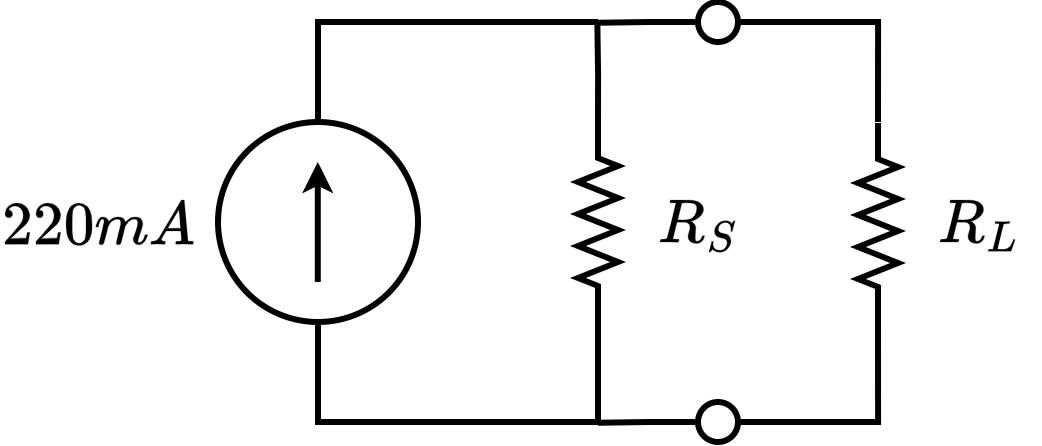
\includegraphics[width=0.5\textwidth]{questionbank/simple_circuits/resistor_search/v1/figure.png}
\end{center}

% =========================================================
\begin{partquestion}{findvalue}
{Find the values for $R_S$ and $R_L$ that satisfy these constraints, assuming the resistors accurately match their marked values.}

\begin{answer}
There are 24 standard resistance values within a decade of values; We only need consider one decade of values for the (smaller) $R_S$ since we will get identical results if we scale each resistor by a factor of ten:
\[
\frac{10R_S}{10R_S + 10R_L} = \frac{R_S}{R_S + R_L}
\]
Since the dissipated current will be of the form $P = I^2R$, we wish to make the resistances as small as possible to minimize this current dissipation, and we restrict our search to $\qty{1}{\ohm} \leq R_S \leq \qty{91}{\ohm}$. After choosing an $R_S$ we can find the optimal $R_L$ through the current divider relationship:
\begin{gather*}
I_L = \frac{R_S}{R_S + R_L}(I_{\text{source}}) \\
R_L = R_S(\frac{I_{\text{source}}}{I_L} - 1) = R_S(\frac{\qty{220}{\milli\ampere}}{\qty{17}{\milli\ampere}} - 1) = 11.941R_S
\end{gather*}
Then we can select an actual resistance value that is closest to $11.941R_S$ and record the deviation. Since this ratio is > 10 we know that $R_L$ must be one decade up. We can manually step through 24 calculations, or we can write a small script to find the best pair. The Python script below is not super-efficient because it looks at every pair of resistors and then sorts them, but it is simple to understand, and the speed of execution is not critical since the search space is so small.

\clearpage
\begin{lstlisting}
 Build the E24 series of resistors
E24 = [10, 11, 12, 13, 15, 16, 18, 20, 22, 24, 27, 30, 33, 36, 39, 43, 47, 51, 56, 62, 68, 75, 82, 91];
# Construct the E24 series of resistors shift down one decade
E24_down = [x / 10 for x in E24]

# Given a target current and load, find the best pair of resistors from the E24 series to achieve that ratio
supply = 0.22;
load = 0.017;
ratio = (supply / load) - 1;

# Build a list of all possible pairs of resistors from the E24 series and their ratios
results = []
for rs in E24_down:
    for rl in E24:
        pair = {
            'rs': rs,
            'rl': rl,
            'ratio': rl / rs
        }
        results.append(pair)

# Sort according to the absolute difference between the target ratio and the calculated ratio, and print the top 5 results
results.sort(key=lambda x: abs(x['ratio'] - ratio))
print("Target ratio: " + f"{ratio:.6f}")
for i in range(5):
    print(str(i + 1) + ": " + str(results[i]['rs']) + " and " + str(results[i]['rl']) + " with ratio " + f"{results[i]['ratio']:.6f}")
\end{lstlisting}

Executing this gives the following output:

\begin{lstlisting}
Target ratio: 11.941176
1: 3.6 and 43 with ratio 11.944444
2: 4.7 and 56 with ratio 11.914894
3: 1.0 and 12 with ratio 12.000000
4: 1.5 and 18 with ratio 12.000000
5: 2.0 and 24 with ratio 12.000000
\end{lstlisting}
So we have $R_S = \qty{3.6}{\ohm}$ and $R_L = \qty{43}{\ohm}$
\end{answer}
\end{partquestion}

% =========================================================
\begin{partquestion}{deviation}
{Calculate the \% deviation from the desired load current}

\begin{answer}
The two resistors above provide a load current of
\[I_L=\frac{\qty{3.6}{\ohm}}{\qty{3.6}{\ohm} + \qty{43}{\ohm}}(\qty{220}{\milli\ampere}) = \qty{16.996}{\milli\ampere}\]
which is a deviation of only
\[\frac{16.996-17}{17}\times100\% \approx0.025\%\]
\end{answer}
\end{partquestion}

% =========================================================
\begin{partquestion}{power}
{Calculate the total power dissipated in the circuit}

\begin{answer}
The total power dissipation is the sum of the power dissipated in each resistor. The current through the source resistor must be $220 - 16.996 = \qty{203.004}{\milli\ampere}$ and we can calculate
\[
P_{\text{total}} = P_{R_s} + P_{R_L} = {I_{R_S}}^2 R_S +{I_{R_L}}^2 R_L = (\qty{0.203}{\ampere})^2(\qty{3.6}{\ohm})+\qty{0.017}{\ampere}^2(\qty{43}{\ohm}) = \qty{0.16}{\watt}
\]
\end{answer}
\end{partquestion}

\end{mainquestion}